\documentclass[10pt,twocolumn]{article}
\usepackage{graphicx}
\usepackage{subfigure}
\usepackage{fancyhdr}
\usepackage{amssymb,amsmath}
\usepackage{nicefrac}
\usepackage[usenames,dvipsnames]{color}
\usepackage[colorlinks,citecolor=RedViolet,urlcolor=blue]{hyperref}
\usepackage{doi}
\usepackage{setspace}
\usepackage[paperwidth=8.5in, paperheight=11in,top=1in, bottom=1in, left=1in, right=1in]{geometry}
\usepackage[compact]{titlesec}
\usepackage{abstract}

\usepackage[authoryear,square]{natbib}
\pagestyle{fancy}
\fancyhead[R]{Veibell \thepage}
\fancyhead[L]{}

\begin{document}
\title{Relationship between solar wind, $D_{st}$, and plasmasphere mass density on one-hour time scales}
\author{
Victoir Veibell\footnote{vveibell@gmu.edu}
\and
R.S. Weigel\footnote{rweigel@gmu.edu}}


\setlength{\parskip}{3ex}
\renewcommand{\labelitemi}{$-$}
\titlespacing{\section}{0pc}{0.2pc}{-1pc}
\titlespacing{\subsection}{0pc}{0.1pc}{-1pc}
\titleformat*{\section}{\normalsize\bfseries}
\titleformat*{\subsection}{\small\bfseries}

\twocolumn[
  \begin{@twocolumnfalse}
\maketitle
\hrule
\begin{abstract}
This paper looks at how various magnetosphere conditions behave around the onset of geomagnetic storms. It confirms results from previous papers that a sudden drop in $D_{st}$ correlates with a spike in equatorial mass density, while adding a level of depth and specification to the applicability of their results. It compares data at 1-hour averages to data at 1-day averages, and briefly to data at 27-day averages to examine if the trend holds at varying time scales and finds that it does, so long as the data is pre-processed to linearly remove a large time scale $F_{10.7}$ dependence. 
\vspace{2em}
\end{abstract}
 \end{@twocolumnfalse}
  ]

\saythanks
% while adding a level of depth and specification to the applicability of their results. It compares data at 1-hour averages to data at 1-day averages, and briefly to data at 27-day averages to examine if the trend holds at varying time scales and finds that it does, so long as the data is pre-processed to linearly remove a large time scale $F_{10.7}$ dependence. 

\section{Introduction}
% try is colloqual.  
% hope is colloqual.
% intends is colloqual.

\cite{Takahashi2010} show that spikes in the Disturbance Storm Time ($D_{st}$) index coincide with with significant changes in $\rho_{eq}$ at an L-shell of 6.8$R_E$. For five storms over a 20 day period two had $\rho_{eq}$ spikes after the $D_{st}$ drop, two had $\rho_{eq}$ spikes before the drop, and one showed little change in $\rho_{eq}$. They then show an epoch analysis where $\rho_{eq}$ is seen to spike the day of a $D_{st}$ drop, using a daily average of 30 minute $\rho_{eq}$ and one hour $D_{st}$ measurements. 

The prior paper, \cite{Takahashi2006}, show how trends in storm dependence on mass/density only appear in longer timescales. Looking at $Kp$ vs mass ($amu$) in the range of 6 to 7 $R_E$, a trend shows up in the 1.5 day averages that doesn't appear in the 3 hour averages.

\cite{Lavraud2006} show that storms preceded by a northward interplanetary magnetic field (IMF) tend to have higher plasma density than those preceded by a southward IMF, and suggest an increased geoeffectiveness from a northward IMF and dense plasma sheet.

\cite{Tsurutani1997} show how the density of a corotating interaction region (CIR) shows strong preconditioning for a drop in $D_{st}$ and spike in magnetic field intensity. Assuming a reasonable amount of coupling between that region's density and the plasmaspheric density, this result could be relatable to others focusing on the plasmasphere. 

\cite{Denton2006} show how $D_{st}$ affects the distribution of plasma density along different magnetic latitudes, and specifically along the same field lines as looked at in later papers (6-8$R_E$). Though this shows that the trends for density may differ between field lines, it's mentioned mostly as a point for future research as the data used in this paper is already adjusted for one field line, as described by \cite{Takahashi2010}.

\cite{Yao2008} looks at the differences in how $D_{st}$ correlates with number density for different ions in different regions (ring current and plasma sheet), but still finds a general correlation during each of the four storms selected.

\section{Previous Results}
We will briefly compare our results to other published results to verify our methods and handling of data. 

Our work takes the datasets from \cite{Denton} and \cite{Reconstruction}, uses a mean interpolation to take the mass density parameter from a highly non-uniform 15 minute grid of the former to the contiguous one hour grid of the latter, and looks for storms based on the definition of storm periods provided by \cite{Takahashi2010}, namely when $D_{st}<-50nT$. The former has a time coverage of 1980-1991, but covered by different satellites in different years (sometimes with overlap), and the latter data set covers 1972-2013. By then looking at an hourly average of variables from 24 hours before storm onset to 48 hours after, short timescale trends can be discerned. 


\section{Data Preparation}
Starting from the data provided by \cite{Denton} for $\rho_{eq}$ and $F_{10.7}$, and \cite{Reconstruction} for all other variables, the data were prepared to get all variables on the same consecutive time-grid. Since the latter was pre-adjusted to have data on a consecutive one-hour grid, the former variables were adjusted to be compatible. First, since the data covers multiple Geostationary Operational Environmental Satellites (GOES), one in particular (GOES 7) was selected to avoid overlapping data points. 

Second, the various forms of "bad data" were converted from their respective set value to NaNs (e.g. 9999 becomes NaN). It was then condensed in range to match the time range from \cite{Reconstruction} down to the same start and end hours, and then interpolated from the GOES 15-minute grid to the one-hour grid by taking the median of all valid non-NaN data points within half an hour to either side of each hour. When no valid points existed in that hour period, a NaN was kept for the sake of the uniform time grid.

The only other point to note in this section: For finding storm times, all NaNs were linearly interpolated out of the data in order to aid in finding storms that may have had their onset point missing. Though this may skew the onset time slightly, it's thought to be less skewed than trying to determine start and end times with the NaNs in place. This interpolation was only used for determining storm times, and not for any analysis.



\section{Results}


\subsection{DST Storm}
Two storm indicators are looked at in this study. The first is looking for a drop in DST below the threshhold of $-50nT$ specified in \cite{Takahashi2010}, dubbed the "onset", and then considering the timeframe a storm until $D_{st}$ passes back above the $-50nT$ threshold. This method finds 669 such periods between May 1983 and August 1991 with an average duration of 9 hours and a median duration of 3 hours. A subset of longer duration storms will be looked at later. Figure \ref{AllData} shows the average values of $B_Z$, $V_{SW}$, $D_{st}$, $F_{10.7}$, and Mass Density for a period of 24 hours before and 48 hours after a storm onset, as well as a plot of mass density with the found storm times highlighted.



This figure shows a definite spike in the $Z$ component of the magnetic field, as well as the defined drop in $DST$, but no obvious change in mass density at an hourly timescale. This points to an issue with only looking at long-timescale trends between density and $D_{st}$, and allows for the possibility that other factors are influencing the long term correlation since there's no obvious connection on a short timescale. One possibility is that, as suggested in \cite{Takahashi2010}, $F_{10.7}$ plays a significant role in driving long term density values which biases the long term correlation of density and $D_{st}$.

\subsection{Mass Density Storm}
Figure \ref{MassStorm} shows this same algorithm, but looking for a rise in mass density over a value of 40$g/cm^3$. This results in 130 storms with a mean duration of 32 hours and a median duration of 17 hours, marked in red on the left figure.



This shows that when using all data for mass density derived storms, almost no significant changes can be seen around storm onset.



\section{More specific storms}
It's hypothesized that progressively picking more specific storm criteria will allow for the possibility of more significant results, at the expense of more bias in the selection process and potentially less overall usefulness of the results. That said, the predictability of extreme storms is of definite interest, so an attempt has been made to find some reproducible method of prediction. Looking at storms that last longer than 12 hours and storms with an onset threshhold greater than $70g/cm^3$ results in the left and right sides of Figure \ref{Mspec} respectively.



Neither of these seem to indicate anything too significant, so looking at $D_{st}$ storms instead to look for something that causes a significant change in Mass Density results in Figure \ref{Dspec}. This shows that by either looking only at $D_{st}$ storms that last longer than an hour (left) or at storms where the onset condition is $D_{st}<-80nT$, a spike in mass density is seen, but also a definite lack of data availability to the point where that spike may be coming from less than five of the total 143 storms. 



Unforunately there are no storms in this time frame that are longer than 12 hours with $D_{st}$ minima lower than $-80nT$ that have existing mass density data around onset, so an analysis of this particular relationship can't be made.

\subsection{Change in $\rho_{eq}$}
If instead of looking for storms based on a threshold of $\rho_{eq}$, we instead look for a certain amount of change in $\rho_{eq}$ as the basis for storm onset, we get Figure \ref{rhochange}.



Both raw change and percent change were done in case of bias towards high or low $\rho_{eq}$ periods, respectively. This shows a distinct lack of correlation in either case to a change in $D_{st}$. The percent change in $\rho_{eq}$ does, however, seem to be preconditioned by changes in $B_z$ and $F_{10.7}$.



\section{F10.7 dependence}
In an effort to analyze the dependence of $\rho_{eq}$ on $F_{10.7}$, a few tests were performed. \cite{Takahashi2010} mention a strong correlation between the two. The long term correlation could be a bias for $D_{st}$'s effects, so a linear model was created, recreating mass density purely from $F_{10.7}$ in the form of $\rho_{eq}(t)=A*F_{10.7}(t)$. This re-created $\rho_{eq}$ shows around a 45\% correlation with the actual $\rho_{eq}$, suggesting a strong influence, while doing the same procedure with $DST$ shows only a 20-25\% correlation. 

Taking this re-created data set and subtracting it from the original should remove the $F_{10.7}$ dependence from the data, and allow for a less biased analysis of the relationship between $D_{st}$ and $\rho_{eq}$. Figure \ref{nof107} shows the stack plot for the reduced $F_{10.7}$, where a more distinct peak after storm onset can be seen. It also shows what that removed trend looks like, of the form $\rho_{eq}-\rho_{eq,F_{10.7}}$.



Similarly, looking at the 1 day averaged data with and without the $F_{10.7}$ dependence, Figure \ref{nof107day} shows that the results of \cite{Takahashi2010} hold only once the dependence has been removed. The 27 day trend couldn't be determined as not enough valid data existed to test it.



\newpage
\footnotesize
\bibliographystyle{vplainnat}

\bibliography{reportbib}

\section{Figures}

\begin{figure}[htp]
\centering
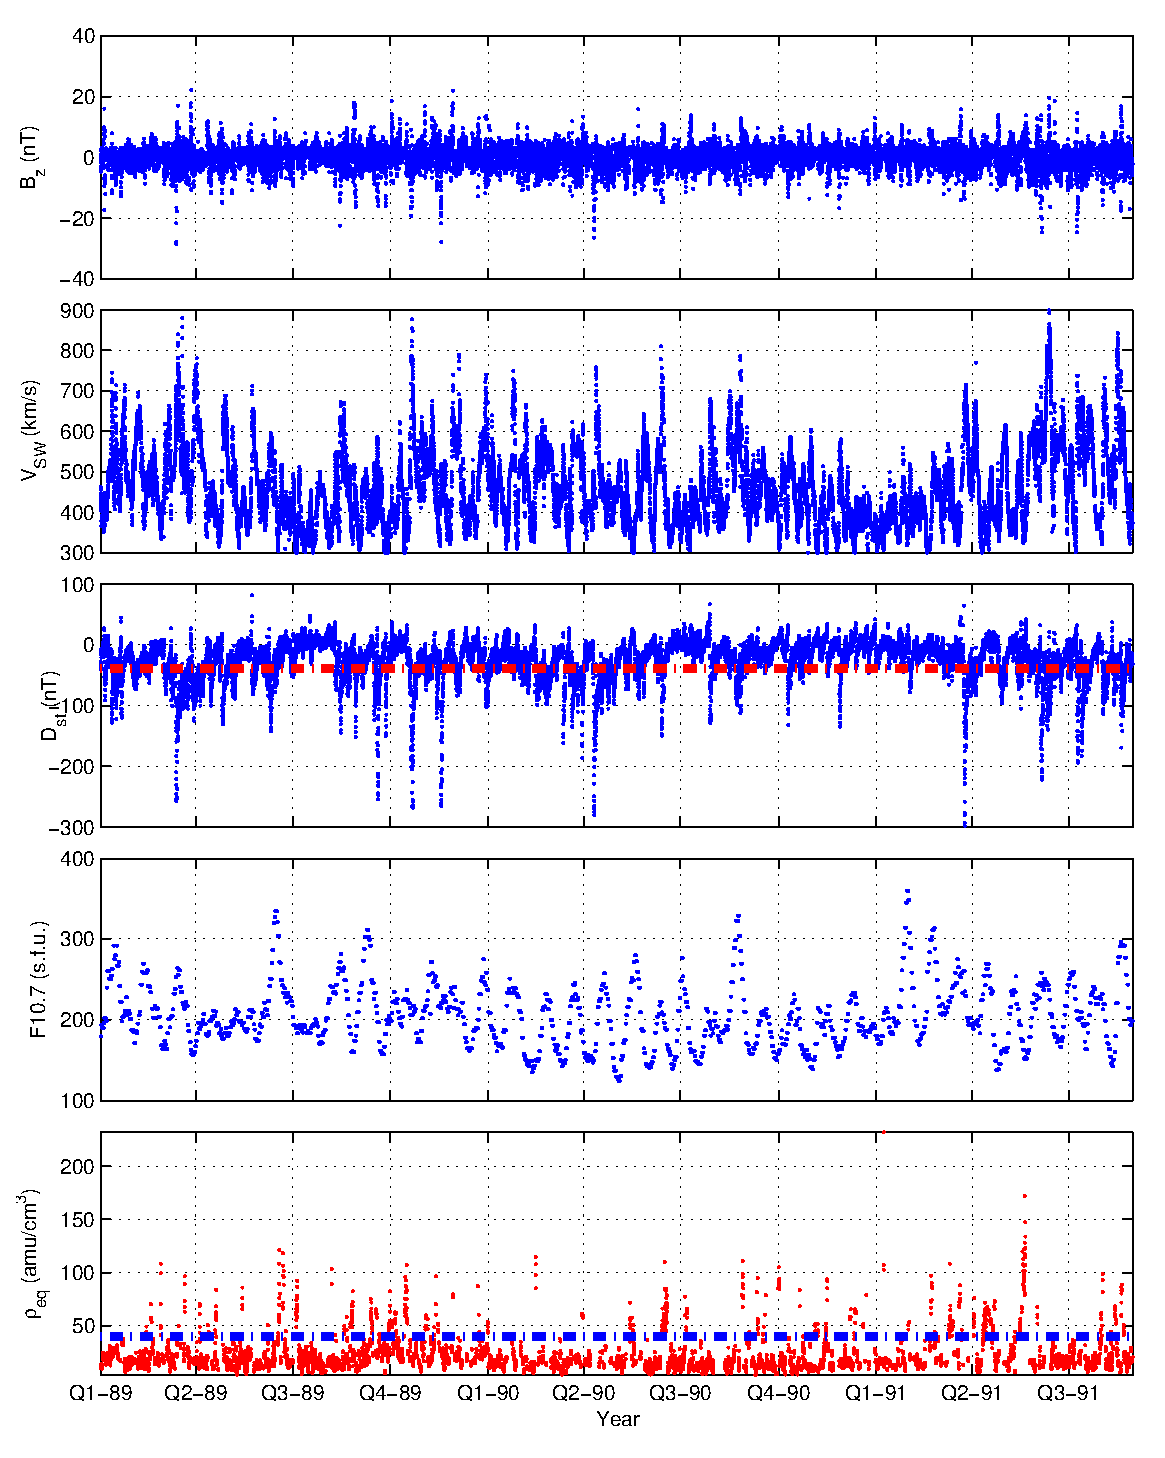
\includegraphics[scale=0.7]{paperfigures/alldata.eps}
\caption{All used data}
\label{AllData}
\end{figure}
\clearpage

\begin{figure}[htp]
\centering
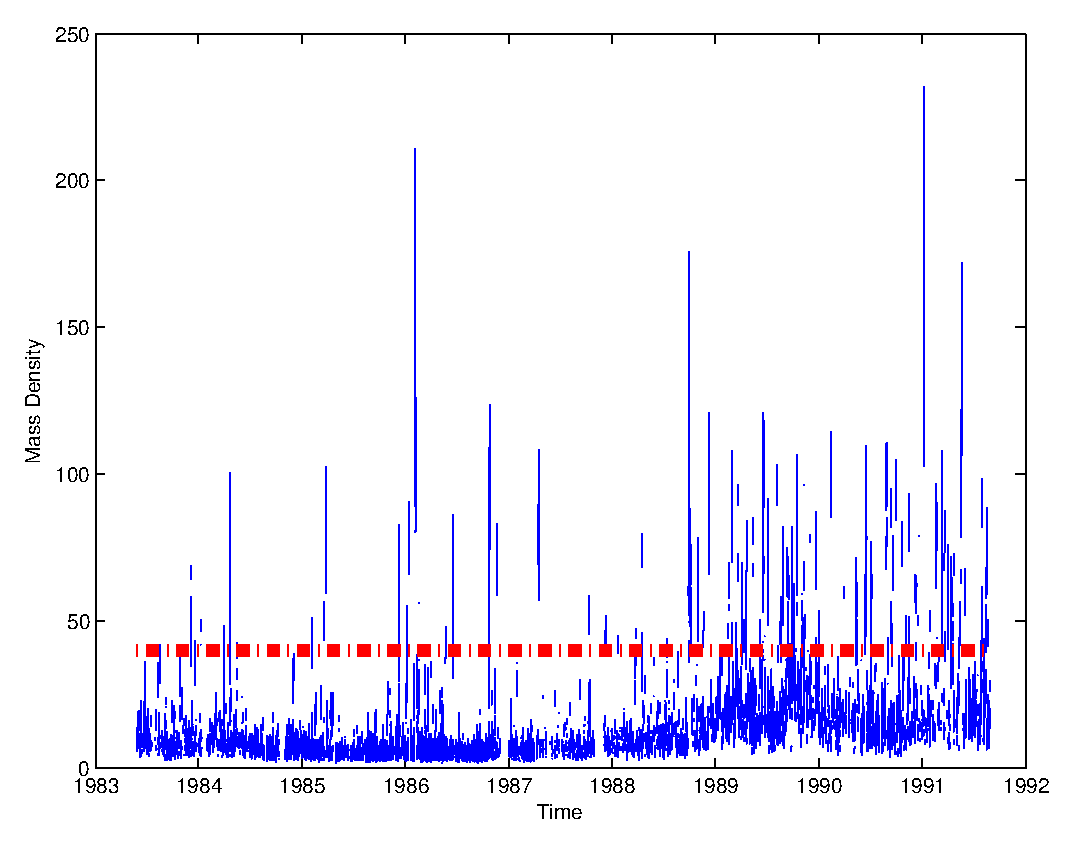
\includegraphics[scale=0.7]{paperfigures/massdensitystorms.eps}
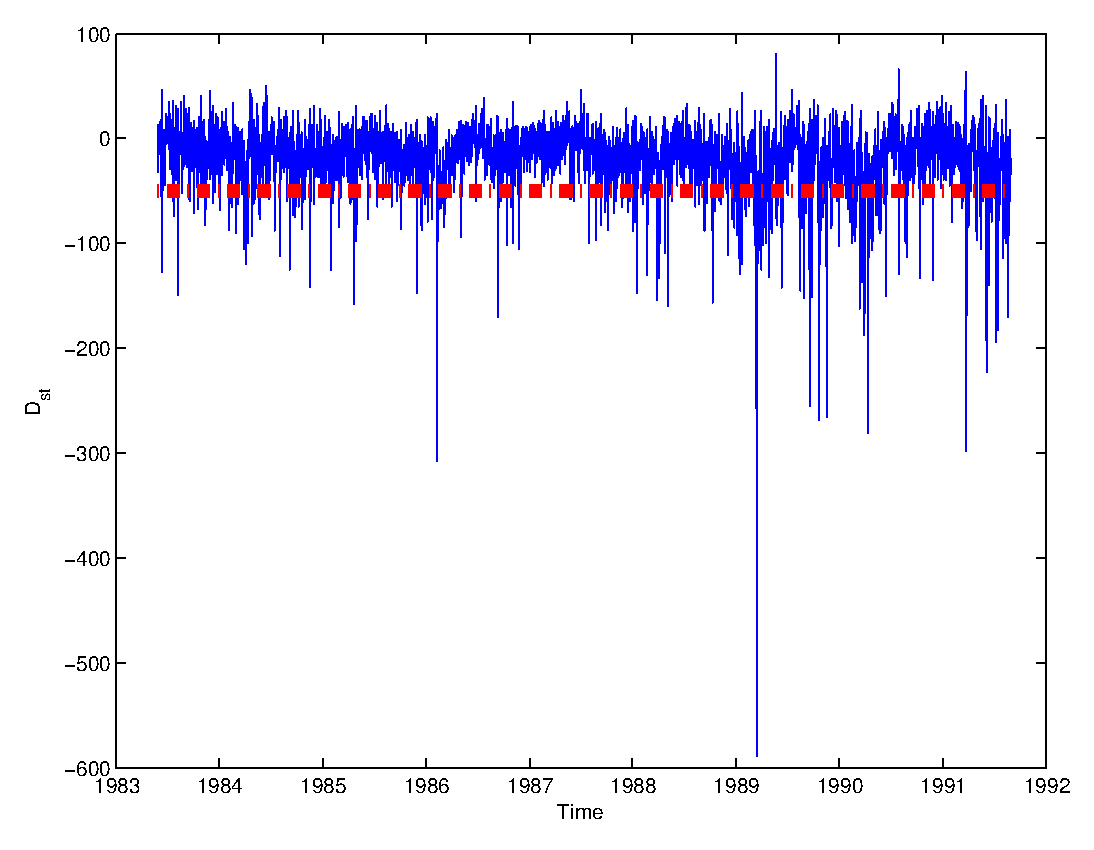
\includegraphics[scale=0.7]{paperfigures/dststorms.eps}
\caption{$\rho_{eq}$ storms (top, red) and $D_{st}$ storm times highlighted (bottom). $\rho_{eq}$ interpolated to 1-hour averages}
\label{DSTstorm}
\end{figure}
\clearpage


\begin{figure}[htp!]
\centering
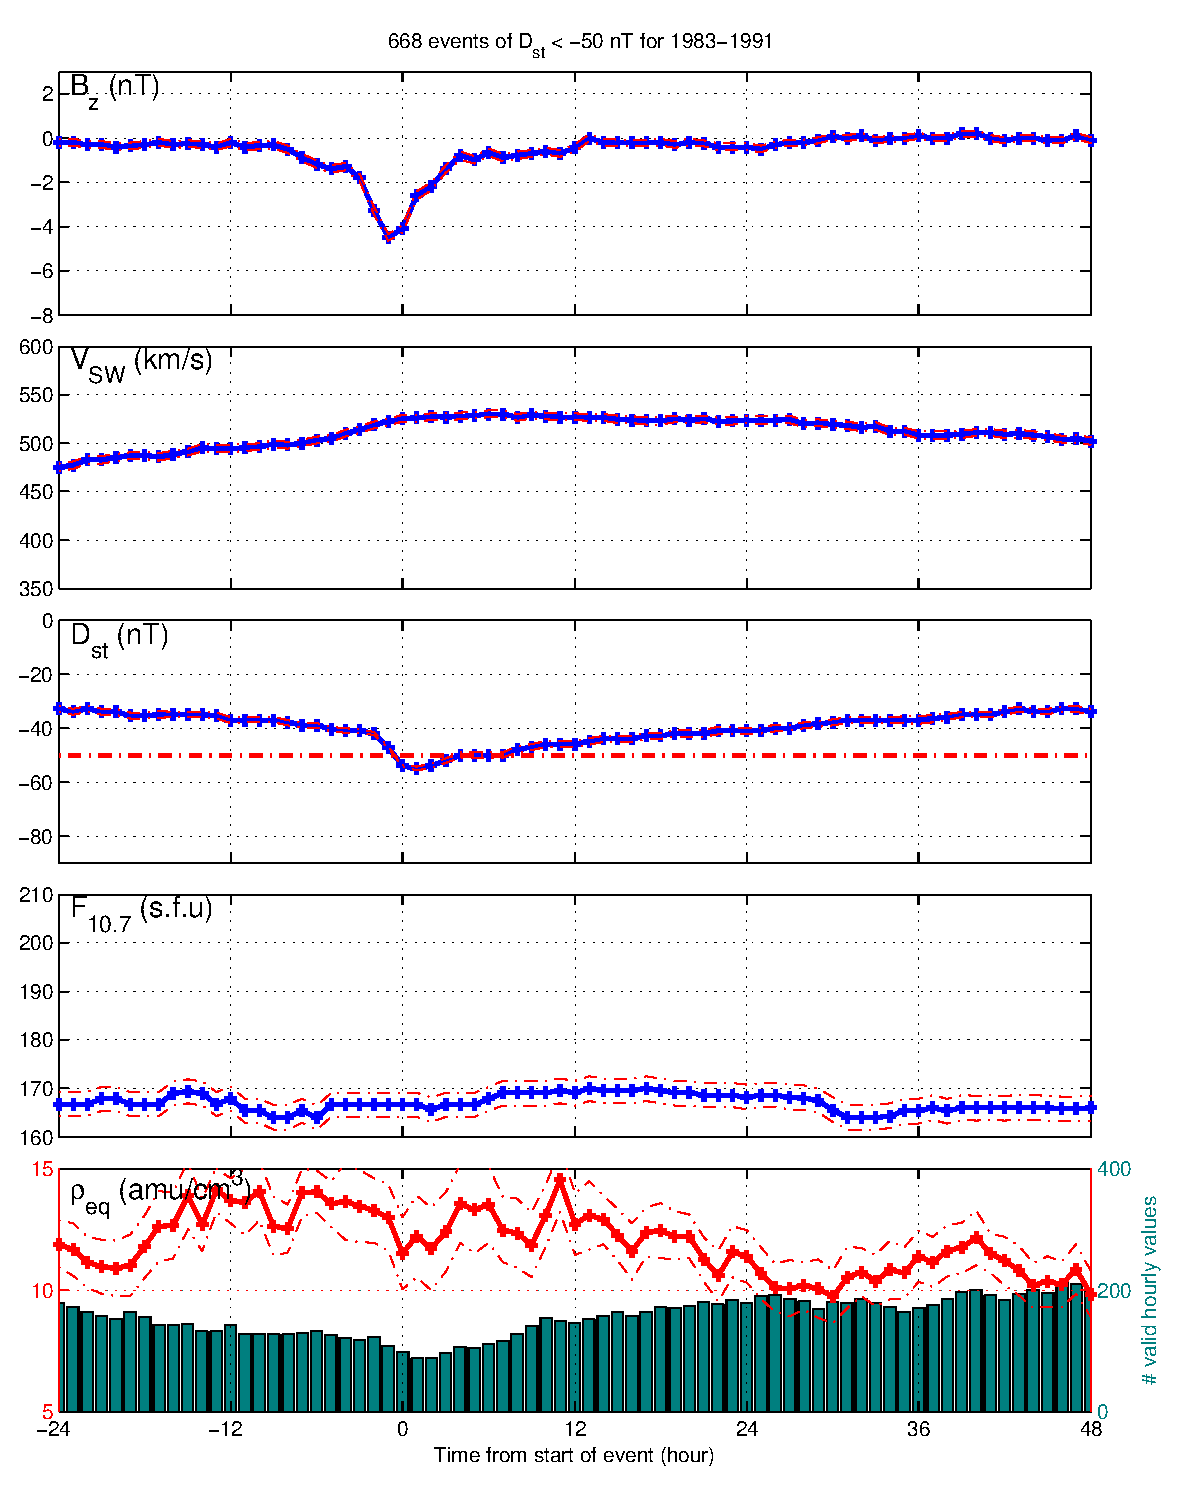
\includegraphics[scale=0.5]{paperfigures/stormavs-dst.eps}
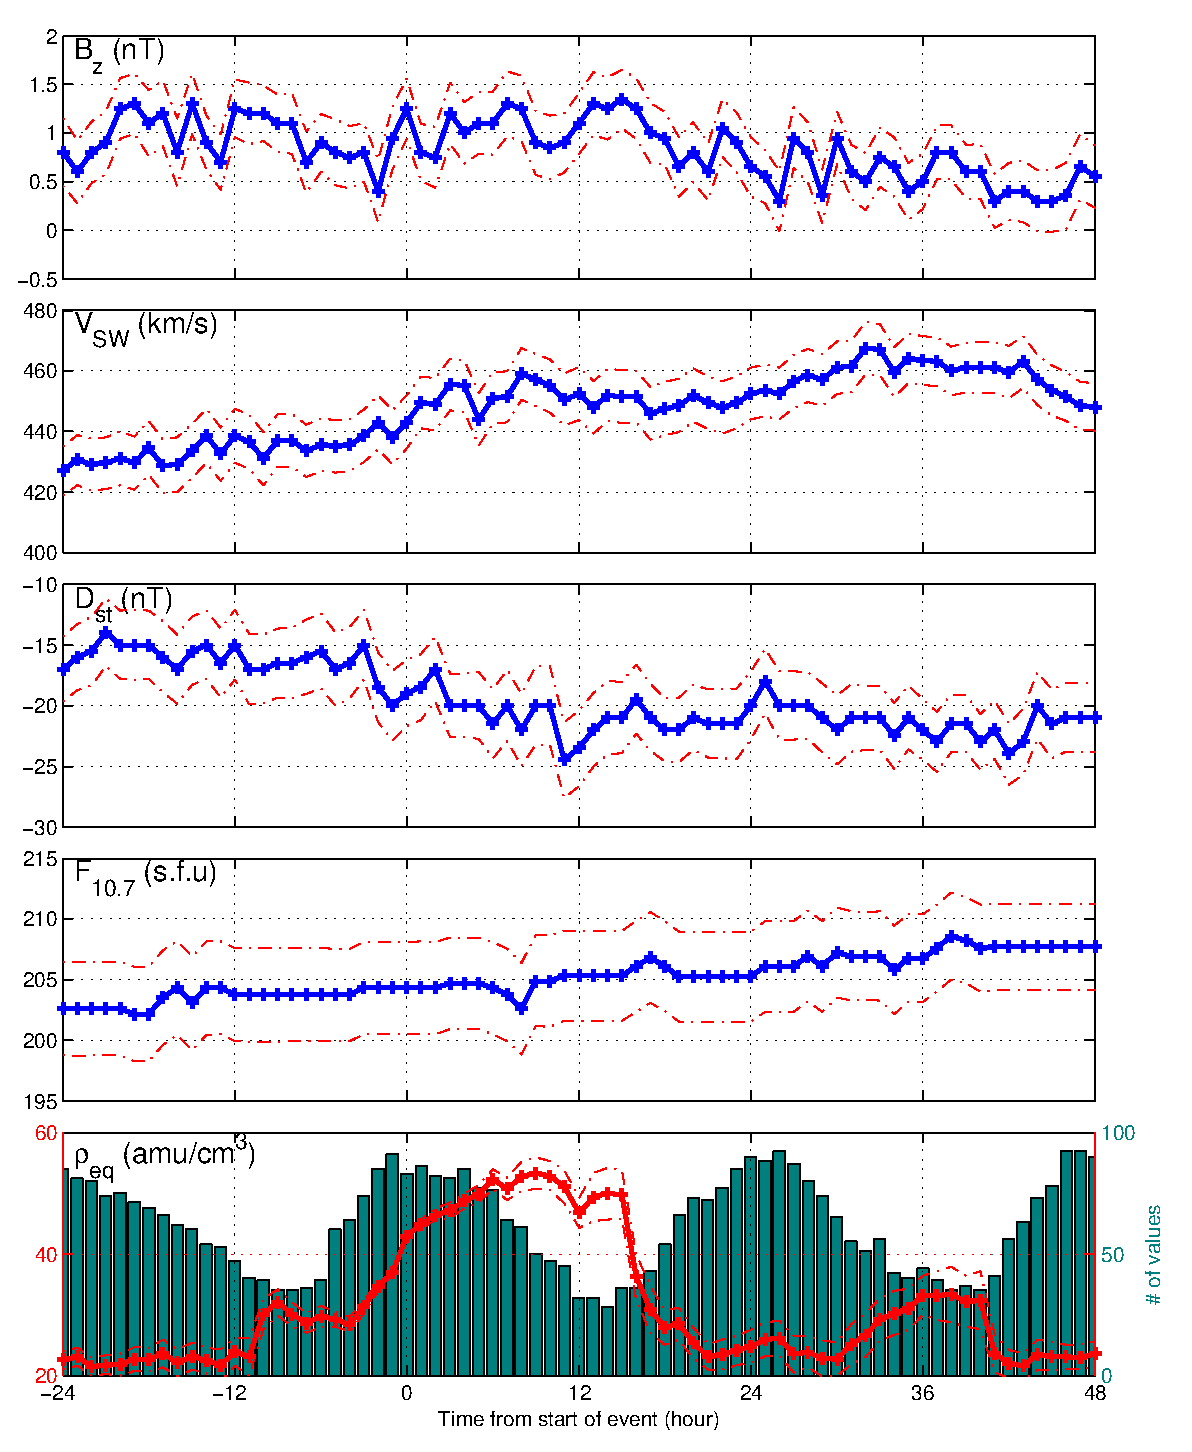
\includegraphics[scale=0.5]{paperfigures/stormavs-mass.eps}
\caption{$D_{st}<-40nT$ onset, Mass Density $>40 amu/cm^3$}
\label{MassStorm}
\end{figure}
\clearpage

\begin{figure}[htp!]
\centering
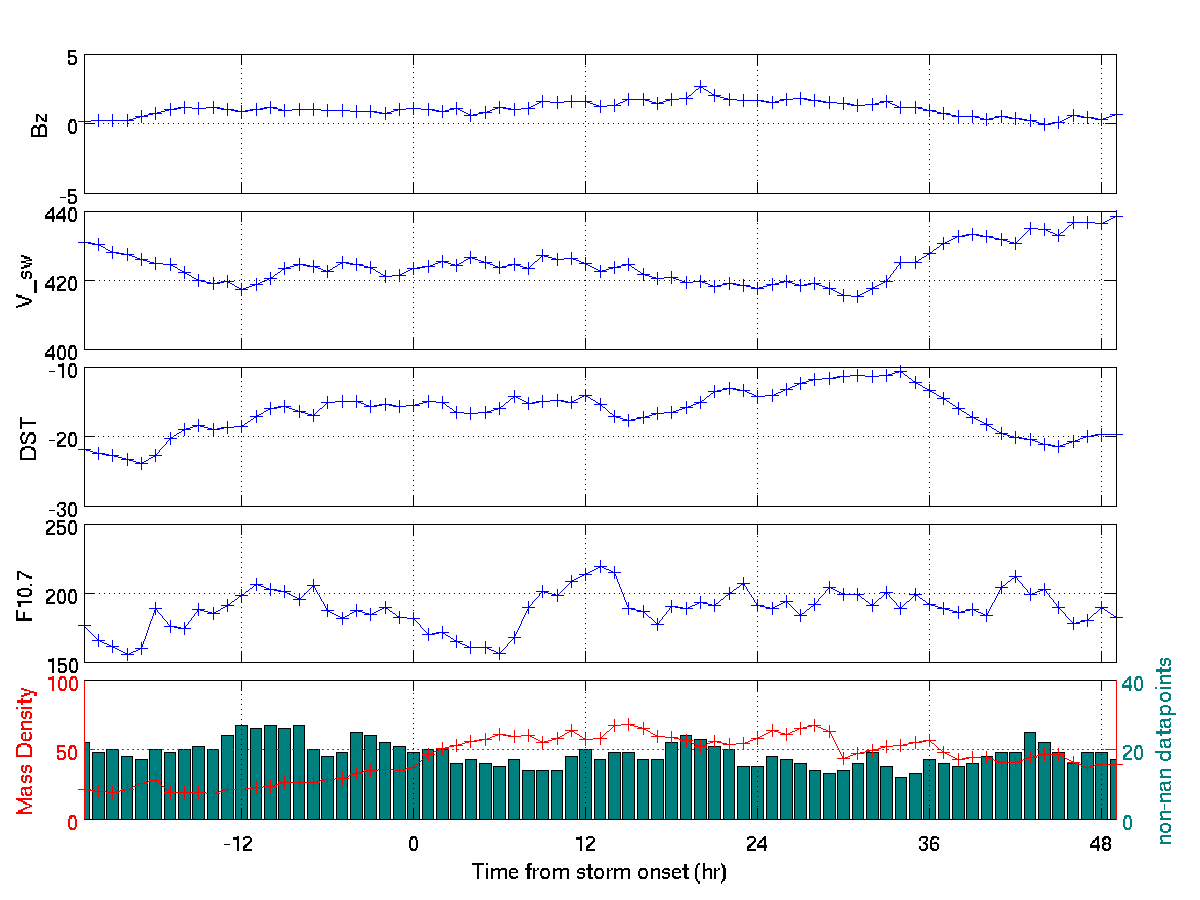
\includegraphics[scale=0.7]{paperfigures/stormavs-md12.png}
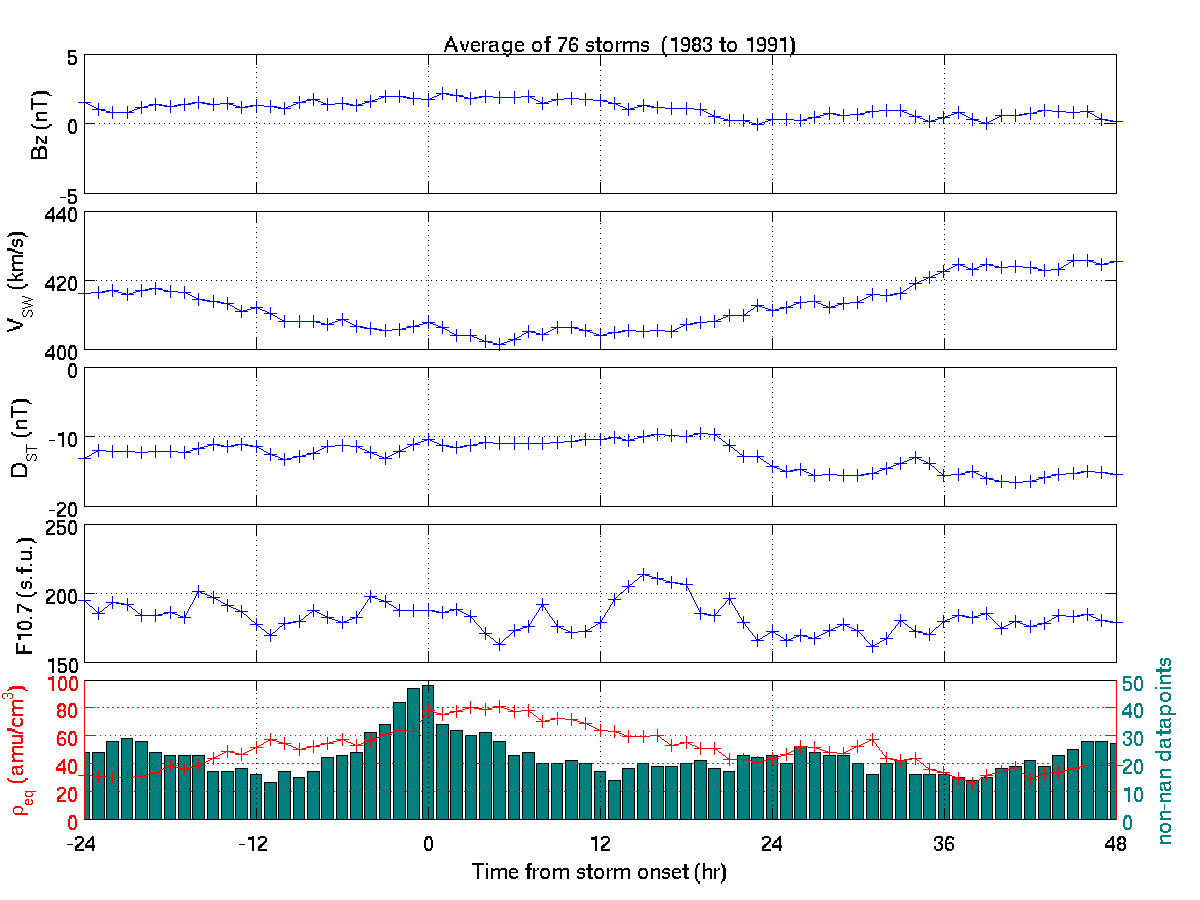
\includegraphics[scale=0.7]{paperfigures/stormavs-m70.png}
\caption{Duration $>$ 12 hours, Mass Density $>70 amu/cm^3$}
\label{Mspec}
\end{figure}
\clearpage

\begin{figure}[htp!]
\centering
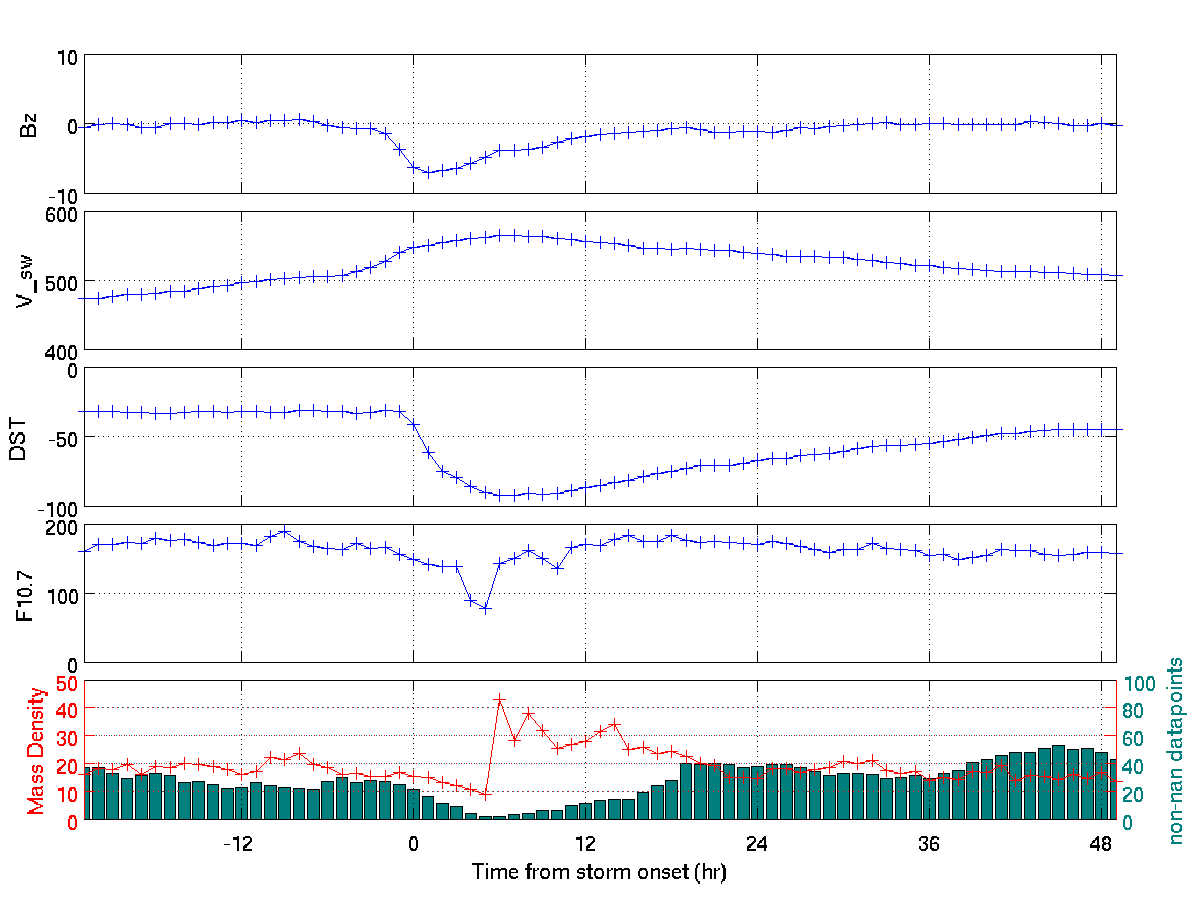
\includegraphics[scale=0.7]{paperfigures/stormavs-dd12.png}
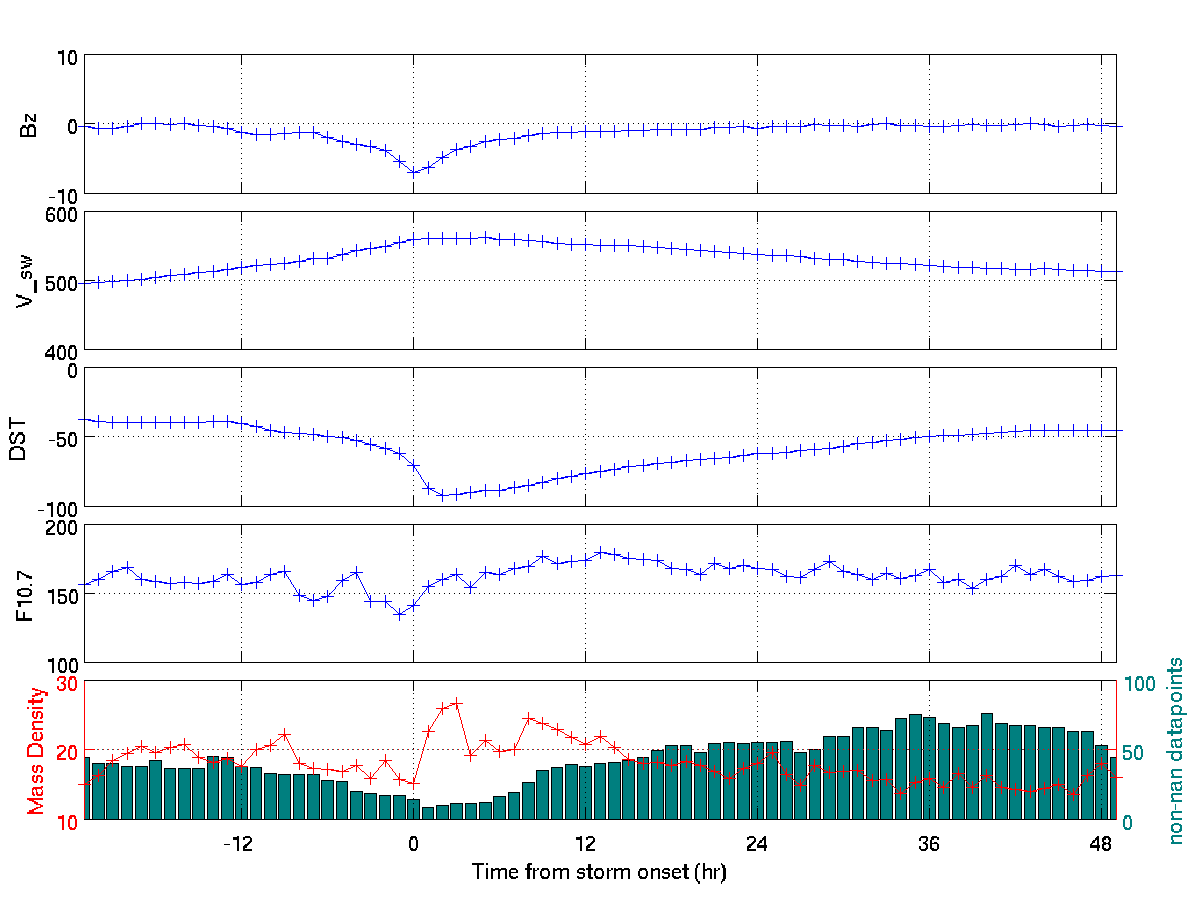
\includegraphics[scale=0.7]{paperfigures/stormavs-d80.png}
\caption{$D_{st}$ Storms $>$ 12 hours, $D_{st}<-80nT$}
\label{Dspec}
\end{figure}
\clearpage

\begin{figure}[htp!]
\centering
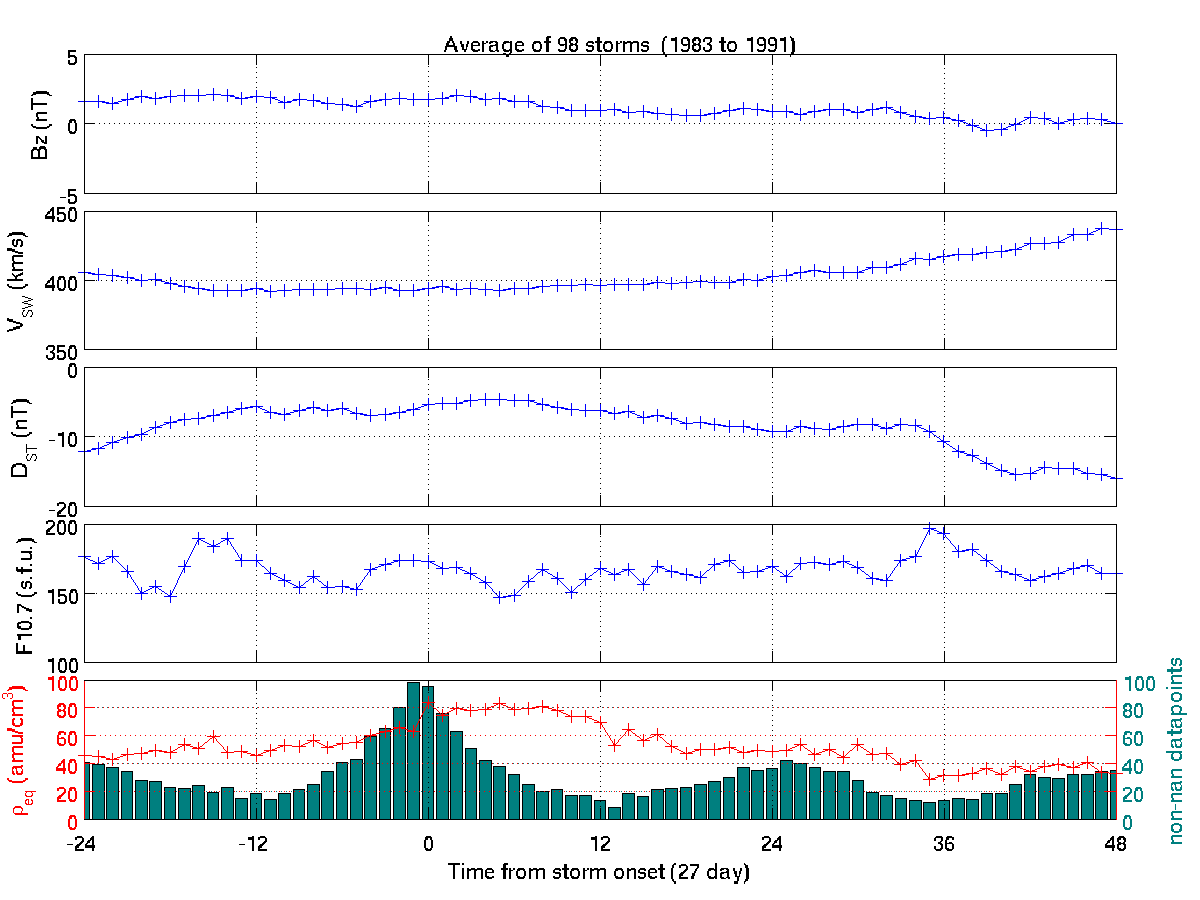
\includegraphics[scale=0.7]{paperfigures/stormavs-diffden-10amu.png}
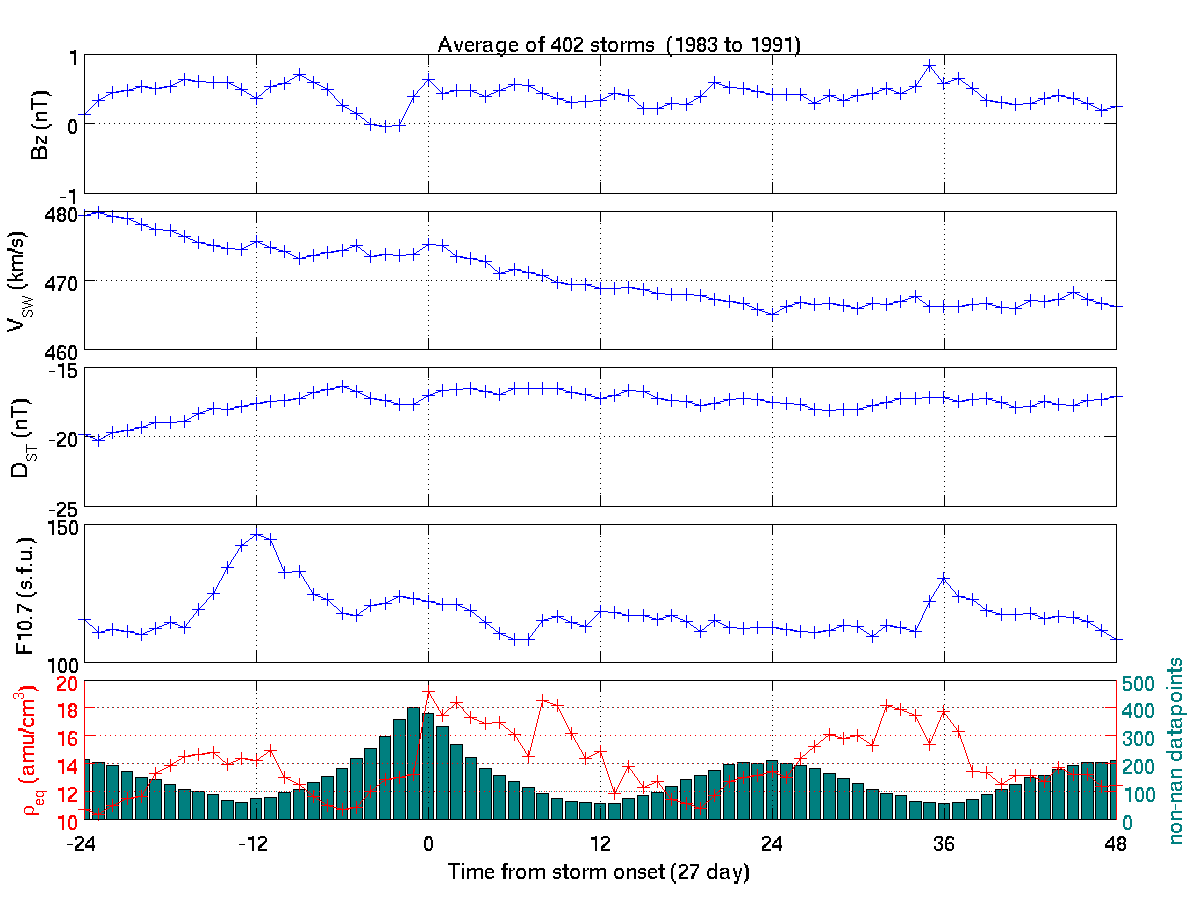
\includegraphics[scale=0.7]{paperfigures/stormavs-diffden-30percent.png}
\caption{diff($\rho_{eq}$) $>$ 20$\frac{amu}{hour}$, diff($\rho_{eq}$) $>$ 30$\frac{\%}{hour}$}
\label{rhochange}
\end{figure}
\clearpage

\begin{figure}[htp!]
\centering
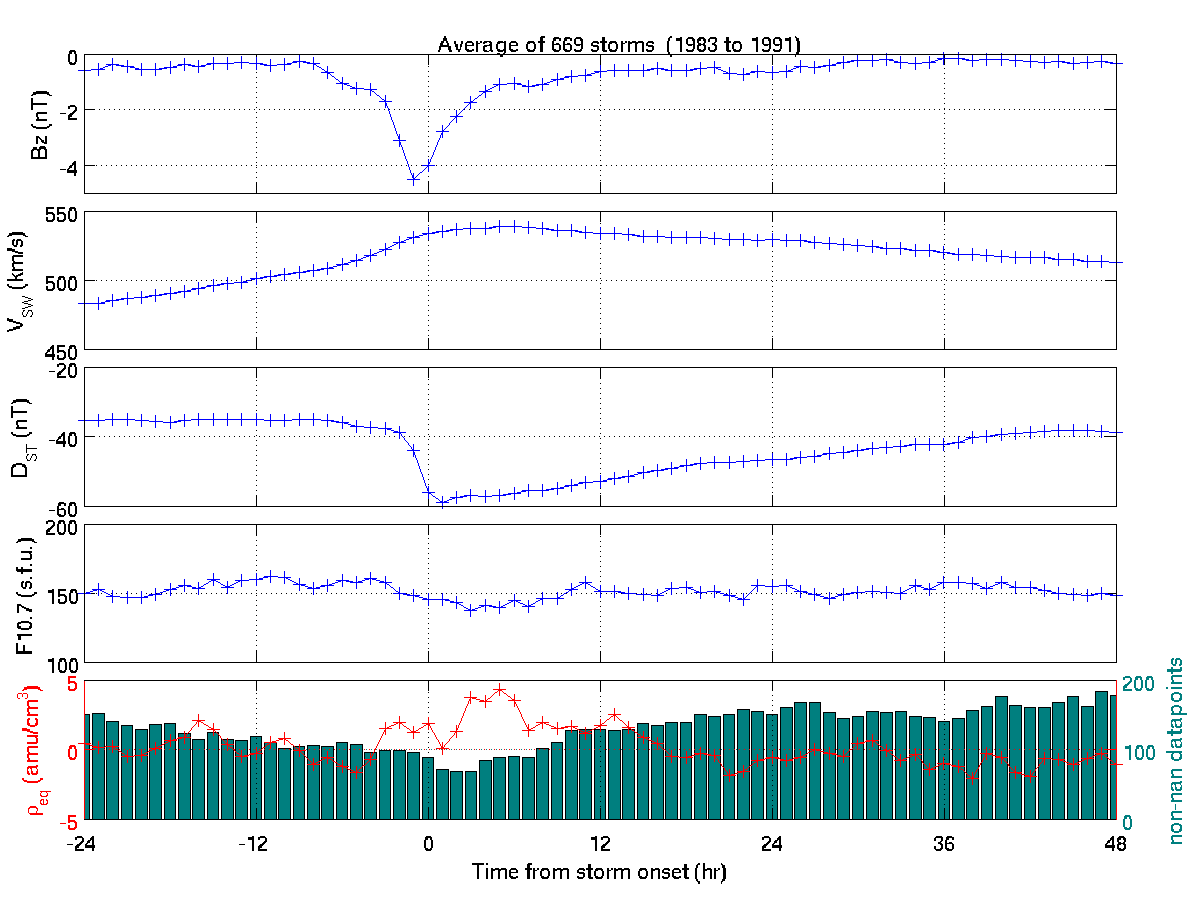
\includegraphics[scale=0.7]{paperfigures/stormavs-dst-nof107.png}
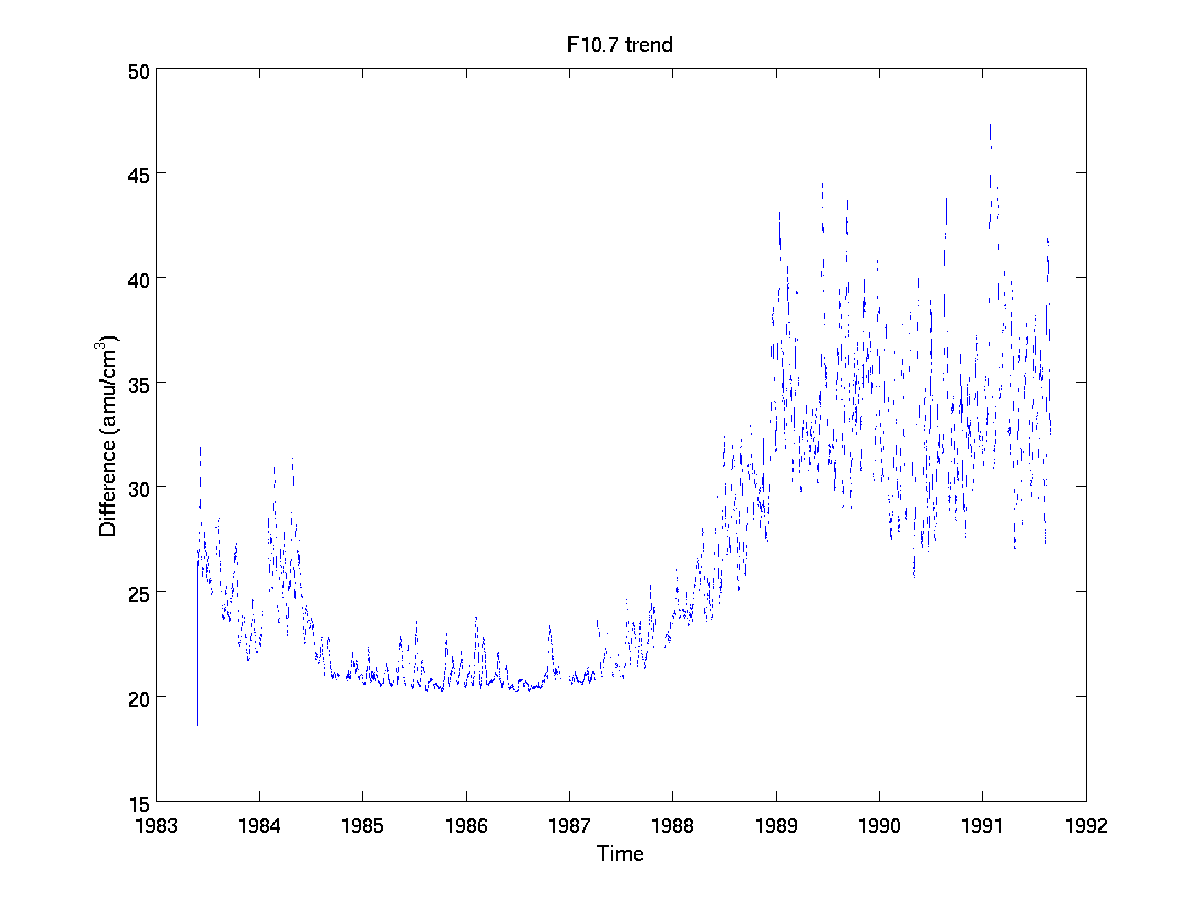
\includegraphics[scale=0.7]{paperfigures/f107removed.png}
\caption{$\rho_{eq}$ with $F_{10.7}$ removed, and Difference from original}
\label{nof107}
\end{figure}
\clearpage

\begin{figure}[htp!]
\centering
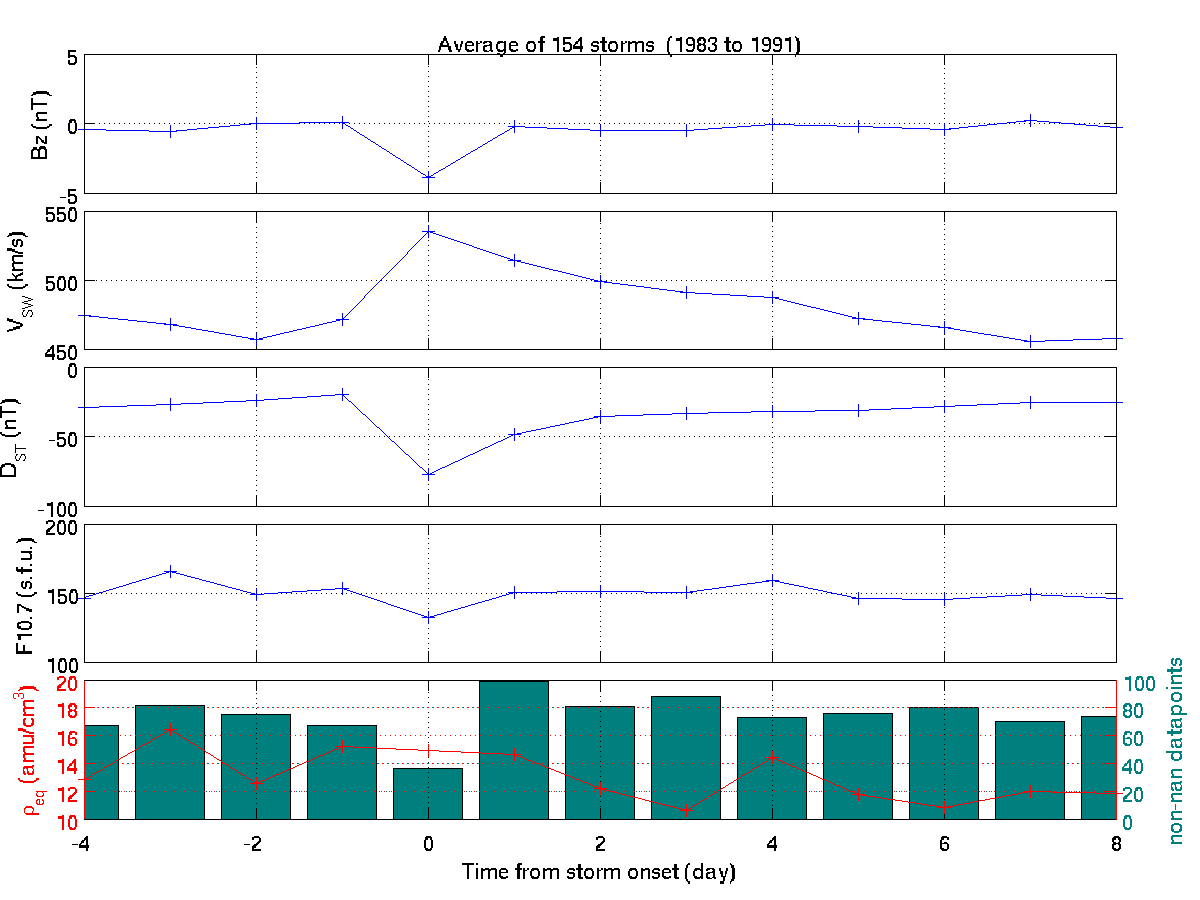
\includegraphics[scale=0.7]{paperfigures/stormavs-dst-day.png}
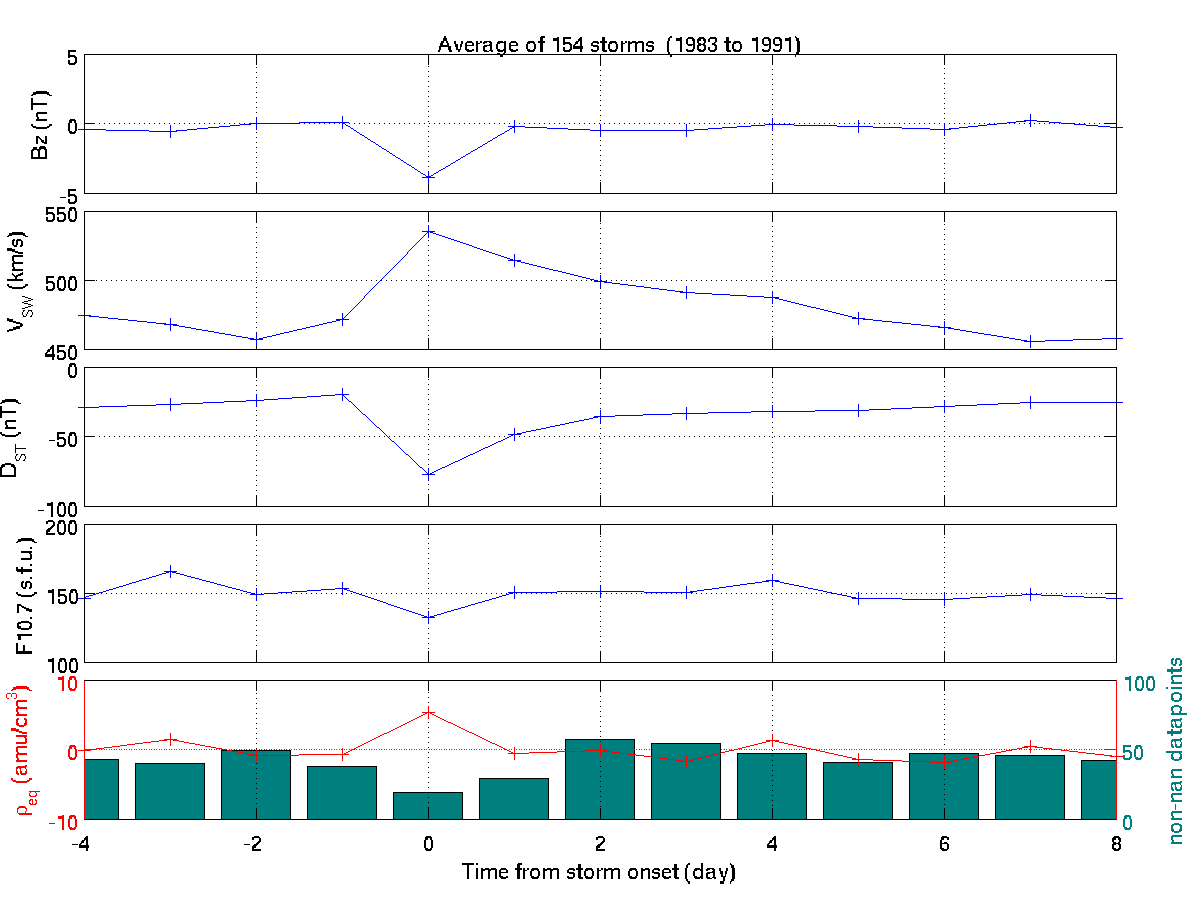
\includegraphics[scale=0.7]{paperfigures/stormavs-dst-day-nof107.png}
\caption{Original $\rho_{eq}$, and with $F_{10.7}$ dependence removed, both at 1-day averages}
\label{nof107day}
\end{figure}

\end{document}
